%%%%%%%%%%%%%%%%%%%%%%%%%%%%%%%%%%%%%%%%%%%%%%%%%%%%%%%%%%%%%%%%%%%%%%%%%%%

\documentclass{standalone}

\usepackage{mathptmx}
\usepackage{tikz}
\usetikzlibrary{external}
\tikzexternalize{circle-octagon}

%% We default to Times.
\renewcommand{\rmdefault}{ptm}
\renewcommand{\ttdefault}{pcr}
%% Enable Times/Palatino main text font.
\normalfont\selectfont

\newcommand{\comma}{,\,}
\newcommand{\tuple}[2]{\left({#1}\comma {#2}\right)}

%% A general circle.
\newcommand{\myCircle}{%%
  %% Draw the circle.
  \draw[lineStyle] (centre) circle[radius=\radius];
  %% Label the centre of the circle.
  \node[nodeStyle] at (centre) {};
  \node at (centre) [below] {$\tuple{0}{0}$};
}

%% An octagon that is inscribed inside a circle.
\newcommand{\myOctagon}{%%
  %% Draw the inscribed octagon.
  \draw[lineStyle] (A) -- (B) -- (C) -- (D) -- (E) -- (F) -- (G)
  -- (H) -- cycle;
  %% Label the corners where the octagon touches the circle.
  %% A
  \node[nodeStyle] at (A) {};
  \node at (A) [right] {$A = \tuple{1}{0}$};
  %% B
  \node[nodeStyle] at (B) {};
  \node at (B) [above right] {$B = \tuple{\frac{\sqrt{2}}{2}}{\frac{\sqrt{2}}{2}}$};
  %% C
  \node[nodeStyle] at (C) {};
  \node at (C) [above] {$C$};
  %% D
  \node[nodeStyle] at (D) {};
  \node at (D) [above left] {$D$};
  %% E
  \node[nodeStyle] at (E) {};
  \node at (E) [left] {$E$};
  %% F
  \node[nodeStyle] at (F) {};
  \node at (F) [below left] {$F$};
  %% G
  \node[nodeStyle] at (G) {};
  \node at (G) [below] {$G$};
  %% H
  \node[nodeStyle] at (H) {};
  \node at (H) [below right] {$H$};
}

%% Approximating pi with an inscribed octagon.

\begin{document}

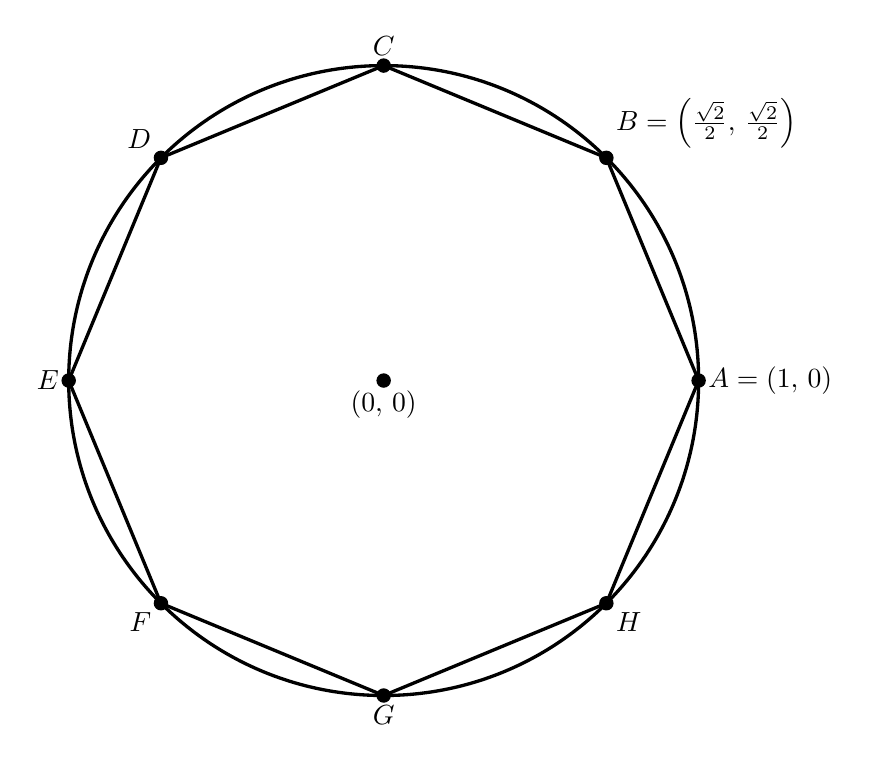
\begin{tikzpicture}[%%
  lineStyle/.style={-,very thick},%%
  nodeStyle/.style={draw,inner sep=1.7pt,circle,fill=black,black}
]
%%
%%
\pgfmathsetmacro{\radius}{4}
\pgfmathsetmacro{\dx}{\radius}
\pgfmathsetmacro{\dy}{\dx}
\pgfmathsetmacro{\xlow}{0}
\pgfmathsetmacro{\ylow}{0}
\coordinate (centre) at (\xlow,\ylow);
%% Coordinates of the octagon.
\coordinate (A) at (\xlow+\dx,0);
\coordinate (B) at (2.82842712474619,2.82842712474619);
\coordinate (C) at (0,\ylow+\dy);
\coordinate (D) at (-2.82842712474619,2.82842712474619);
\coordinate (E) at (\xlow-\dx,0);
\coordinate (F) at (-2.82842712474619,-2.82842712474619);
\coordinate (G) at (0,\ylow-\dy);
\coordinate (H) at (2.82842712474619,-2.82842712474619);
%%
%% Draw a circle with an inscribed square.
\myCircle
\myOctagon
\end{tikzpicture}

\end{document}
